% Kopfzeile beim Kapitelanfang:
\fancypagestyle{plain}{
%Kopfzeile links bzw. innen
\fancyhead[L]{\calligra\Large Vorlesung Nr. 23}
%Kopfzeile rechts bzw. außen
\fancyhead[R]{\calligra\Large 14.01.2013}
}
%Kopfzeile links bzw. innen
\fancyhead[L]{\calligra\Large Vorlesung Nr. 23}
%Kopfzeile rechts bzw. außen
\fancyhead[R]{\calligra\Large 14.01.2013}
% **************************************************
%
\wdh
\enum{
\item Integration der Treppenfunktion % GRAPH Treppenfunktion
\\*
(leicht)
\item $f: [a, b] \to \R$ beschränkt\\
$\int_a^b {}_* f(x) = sup \left\lbrace \int_a^b g(x)dx \mid g: [a,b] \to \R Treppenfunktion, g \leq f \right\rbrace$\\*
$inf \left\lbrace \int_a^b h(x) dx \mid h: f \leg h \right\rbrace = int_a^b {}^* f(x)$
% Mittelwertintegral Graph 
$f$ \ul{integrierbar} wenn $\int_a^b{}_* f(x)dx=\int_a^b{}^* f(x)dx$, dann $\int_a^b{} f(x)dx:=\int_a^b{}_* f(x)dx$
\enum{
\item $f:[a,b]→\R$ stetig \Rarr\ integrierbar
\item Mittelwertsatz: Wenn $f:[a,b]→\R$ stetig, dann gibt es ein $x_0\in[a,b]$ mit $\int_a^b f(x)dx=f(x_0)·(b-a)$\\*
(Grundlage aller Berechnungen)
%Graph mit fläche
}
}

% Treppengraph, erste Tafel
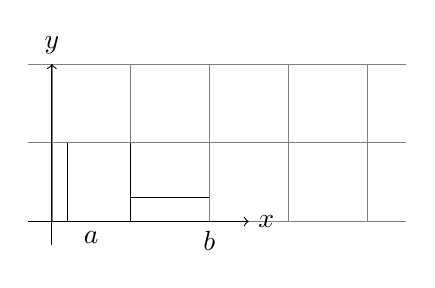
\begin{tikzpicture}
\draw[very thin,color=gray] (-0.3,0.0) grid (4.5,2.0);
\draw[->] (-0.3,0) -- (2.5,0) node[right] {$x$};
\draw[->] (0,-0.3) -- (0,2) node[above] {$y$};
\draw (0.5,0) node[anchor=north] {$a$};
\draw (2,0) node[anchor=north] {$b$};
% Schrafierung einfügen
\draw (0.2, 1) -- (0.2, 1);
\draw (0.2, 0) - - (0.2, 1);
\draw (1, 0) - - (1, 1);
\draw (1, 0.3) -- (2, 0.3);
\end{tikzpicture}\\*

% Graph an der dritten Tafel mit schrafur.
\begin{tikzpicture}[domain=0.5:2,prefix=plots/, smooth]
\draw[very thin,color=gray] (-0.3,0.0) grid (2.5,2.0);
\draw[->] (-0.3,0) -- (2.5,0) node[right] {$x$};
\draw[->] (0,-0.3) -- (0,2) node[above] {$y$};
\draw (0.5,0) node[anchor=north] {$a$};
\draw (2,0) node[anchor=north] {$x-h$};
\draw (0.5, 0) -- (0.5, 1.5);
\draw (2,0) -- (2, 0.6);
\draw[color=blue] plot[id=23.1_int2] function{sin(2x+0.5)} node[below, midway] {};
\end{tikzpicture}\\*

\begin{tikzpicture}[domain=0:2,prefix=plots/, smooth]
\draw[very thin,color=gray] (-0.3,0.0) grid (2.5,2.0);
\draw[->] (-0.3,0) -- (2.5,0) node[right] {$x$};
\draw[->] (0,-0.3) -- (0,2) node[above] {$y$};
\draw[color=black] plot[id=23.2_int] function[cos(x)+1] \node[below, midway] {$f(x)$};
\draw[color=green] (0, 2) -- (0.5, 2);
\draw[color=green] (0.5, 2) -- (0.5, 1.87);
\draw[color=green] (0.5, 1.87) -- (1, 1.87);
\draw[color=green] (1, 1.87) -- (1, 1.54);
\draw[color=green] (1, 1.54) -- (1.5, 1.54);
\draw[color=green] (1.5, 1.54) -- (1.5, 1.07);
\draw[color=green] (1.5, 1.07) -- (2, 1.07);
\draw[color=green] (2, 1.07) -- (2.5, 1.07);
\draw[color=green] (2.5, 1.07) -- (2.5, 0.2);
\draw[color=green] (2.5, 0.2) -- (3, 0.2);
\draw[color=green] (3, 0.2) -- (3.5, 0.1);
\end{tikzpicture}\\*


% Stefan
Grundprinzip:\\*
Jede Ableitungsregel gibt eine Integrationsregel:
\itm{
\item Kettenregel $\to$ Substitutionsregel
\item Produktregel $\to$ Partielle Integration
}

$F(\phi(X)) \mid_a^b = \int_a^b (F(\phi \circ F)'(x)) dx = \int_a^b f(\phi (x)) \cdot \phi'(x)dx$
\bsp
\enum{
\item $\int_a^b f(x + c)dx = \int_a^b \underbrace{f(\phi(t))}_f(t+c) \cdot \underbrace{\phi'(t)}_{=1} dt) = \int_{a + c}^{b + c} f(x) dx$\\*
$\phi(t) = t + c$
$\phi'(t) = 1$
\item $\int_a^b f(c \cdot x) = \int_a^b f(\phi(t)) \cdot \frac{\phi'(t)}{c}dt = \frac{1}{c} \cdot \int_a^b f(x) dx$
}